% answers.tex —— 2006 年·上海春季招生数学试卷 · 参考答案与详细解析片段
% 由 tools/generate_projects.py 依来源总账自 2006/2006_数学真题_春季上海_试题.md + 2006/2006_数学真题_春季上海_解析正文.md + 2006/2006_数学真题_春季上海_答案要点.md 生成，勿手改（改源 MD 后重跑）


\begin{gktip}
以下答案与解法根据固定来源第 1–2 页的题面独立推导。扫描副本第 2–4 页另印“参考答案”与解答，但发布者、版本和官方身份未核；对应转录见源载参考答案稿。题目第 17、20、21 题的数学图将按题面源图语义另行矢量重绘，本文不嵌入扫描页。
\end{gktip}

\begin{answer}
\gksolhead{1}{}

\textbf{题目}：

计算：$\displaystyle\lim_{n\to\infty}\frac{3n-2}{4n+3}=\underline{\qquad}$。

\Needspace{4\baselineskip}
\textbf{解析}

\Needspace{5\baselineskip}
分子、分母同除以 $n$，得
\nopagebreak[4]
\[
\lim_{n\to\infty}\frac{3n-2}{4n+3}
=\lim_{n\to\infty}\frac{3-2/n}{4+3/n}=\frac34.
\]

\gkanswer{答案：$\dfrac34$}

\end{answer}
\begin{answer}
\gksolhead{2}{}

\textbf{题目}：

方程 $\log_3(2x-1)=1$ 的解 $x=\underline{\qquad}$。

\Needspace{4\baselineskip}
\textbf{解析}

由 $\log_3(2x-1)=1$，得 $2x-1=3$，所以 $x=2$，且满足定义域 $2x-1>0$。

\gkanswer{答案：$2$}

\end{answer}
\begin{answer}
\gksolhead{3}{}

\textbf{题目}：

函数 $f(x)=3x+5$，$x\in[0,1]$ 的反函数 $f^{-1}(x)=\underline{\qquad}$。

\Needspace{4\baselineskip}
\textbf{解析}

\Needspace{5\baselineskip}
设 $y=3x+5$，则 $x=(y-5)/3$。原函数在 $[0,1]$ 上的值域为 $[5,8]$，故
\nopagebreak[4]
\[
f^{-1}(x)=\frac{x-5}{3},\qquad x\in[5,8].
\]

\gkanswer{答案：$\dfrac{x-5}{3}$，$x\in[5,8]$}

\end{answer}
\begin{answer}
\gksolhead{4}{}

\textbf{题目}：

不等式 $\displaystyle\frac{1-2x}{x+1}>0$ 的解集是 $\underline{\qquad}$。

\Needspace{4\baselineskip}
\textbf{解析}

\Needspace{5\baselineskip}
临界点为 $x=-1$ 与 $x=\dfrac12$。分式在 $(-1,\dfrac12)$ 为正，端点因分母为零或严格不等号而不取；故
\nopagebreak[4]
\[
\frac{1-2x}{x+1}>0\quad\Longleftrightarrow\quad x\in\left(-1,\frac12\right).
\]

\gkanswer{答案：$\left(-1,\dfrac12\right)$}

\end{answer}
\begin{answer}
\gksolhead{5}{}

\textbf{题目}：

已知圆 $C:(x+5)^2+y^2=r^2\ (r>0)$ 和直线 $l:3x+y+5=0$。若圆 $C$ 与直线 $l$ 没有公共点，则 $r$ 的取值范围是 $\underline{\qquad}$。

\Needspace{4\baselineskip}
\textbf{解析}

\Needspace{5\baselineskip}
圆心为 $(-5,0)$。圆心到直线 $3x+y+5=0$ 的距离为
\nopagebreak[4]
\[
d=\frac{|3(-5)+5|}{\sqrt{3^2+1^2}}=\sqrt{10}.
\]
圆与直线没有公共点要求半径严格小于该距离；结合 $r>0$，得 $0<r<\sqrt{10}$。

\gkanswer{答案：$(0,\sqrt{10})$}

\end{answer}
\begin{answer}
\gksolhead{6}{}

\textbf{题目}：

已知函数 $f(x)$ 是定义在 $(-\infty,+\infty)$ 上的偶函数。当 $x\in(-\infty,0)$ 时，$f(x)=x-x^4$，则当 $x\in(0,+\infty)$ 时，$f(x)=\underline{\qquad}$。

\Needspace{4\baselineskip}
\textbf{解析}

\Needspace{5\baselineskip}
当 $x>0$ 时，偶函数性质给出 $f(x)=f(-x)$。将 $-x$ 代入已知式，得
\nopagebreak[4]
\[
f(x)=(-x)-(-x)^4=-x-x^4.
\]

\gkanswer{答案：$-x-x^4$}

\end{answer}
\begin{answer}
\gksolhead{7}{}

\textbf{题目}：

电视台连续播放 6 个广告，其中含 4 个不同的商业广告和 2 个不同的公益广告，要求首尾必须播放公益广告，则共有 $\underline{\qquad}$ 种不同的播放方式（结果用数值表示）。

\Needspace{4\baselineskip}
\textbf{解析}

两条不同的公益广告分别排在首尾，有 $2!$ 种排法；4 条不同的商业广告排在中间，有 $4!$ 种排法。因此共有 $2!\cdot4!=48$ 种。

\gkanswer{答案：$48$ 种}

\end{answer}
\begin{answer}
\gksolhead{8}{}

\textbf{题目}：

正四棱锥底面边长为 4，侧棱长为 3，则其体积为 $\underline{\qquad}$。

\Needspace{4\baselineskip}
\textbf{解析}

\Needspace{5\baselineskip}
正方形底面中心到一个顶点的距离为 $\dfrac{4\sqrt2}{2}=2\sqrt2$。棱锥高为 $\sqrt{3^2-(2\sqrt2)^2}=1$，故体积为
\nopagebreak[4]
\[
V=\frac13\cdot4^2\cdot1=\frac{16}{3}.
\]

\gkanswer{答案：$\dfrac{16}{3}$}

\end{answer}
\begin{answer}
\gksolhead{9}{}

\textbf{题目}：

在 $\triangle ABC$ 中，已知 $BC=8$，$AC=5$，三角形面积为 12，则 $\cos 2C=\underline{\qquad}$。

\Needspace{4\baselineskip}
\textbf{解析}

\Needspace{5\baselineskip}
由三角形面积公式，$12=\dfrac12\cdot AC\cdot BC\cdot\sin C$，所以 $\sin C=\dfrac35$。于是
\nopagebreak[4]
\[
\cos2C=1-2\sin^2C=1-2\cdot\frac9{25}=\frac7{25}.
\]

\gkanswer{答案：$\dfrac7{25}$}

\end{answer}
\begin{answer}
\gksolhead{10}{}

\textbf{题目}：

若向量 $\vec a,\vec b$ 的夹角为 $150^\circ$，$|\vec a|=\sqrt3$，$|\vec b|=4$，则 $|2\vec a+\vec b|=\underline{\qquad}$。

\Needspace{4\baselineskip}
\textbf{解析}

\Needspace{5\baselineskip}
利用向量数量积，
\nopagebreak[4]
\[
\begin{aligned}
|2\vec a+\vec b|^2
&=4|\vec a|^2+|\vec b|^2+4\vec a\cdot\vec b\\
&=12+16+4\cdot\sqrt3\cdot4\cos150^\circ\\
&=12+16-24=4.
\end{aligned}
\]
因此 $|2\vec a+\vec b|=2$。

\gkanswer{答案：$2$}

\end{answer}
\begin{answer}
\gksolhead{11}{}

\textbf{题目}：

已知直线 $l$ 过点 $P(2,1)$，且与 $x$ 轴、$y$ 轴的正半轴分别交于 $A\text{、}B$ 两点，$O$ 为坐标原点，则三角形 $OAB$ 面积的最小值为 $\underline{\qquad}$。

\Needspace{4\baselineskip}
\textbf{解析}

\Needspace{5\baselineskip}
设直线 $l$ 与正半轴的截距分别为 $A=(u,0)$、$B=(0,v)$，其中 $u,v>0$。由截距式及 $P(2,1)\in l$，有 $\dfrac2u+\dfrac1v=1$，于是 $u>2$ 且 $v=\dfrac{u}{u-2}$。三角形面积
\nopagebreak[4]
\[
S=\frac{uv}{2}=\frac{u^2}{2(u-2)}.
\]
由 $\dfrac{u^2}{u-2}-8=\dfrac{(u-4)^2}{u-2}\geq0$，得 $S\geq4$；当 $u=4$、$v=2$ 时取等号。

\gkanswer{答案：$4$}

\end{answer}
\begin{answer}
\gksolhead{12}{}

\textbf{题目}：

\Needspace{5\baselineskip}
同学们都知道，在一次考试后，如果按顺序去掉一些高分，那么班级的平均分将降低；反之，如果按顺序去掉一些低分，那么班级的平均分将提高。这两个事实可以用数学语言描述为：若有限数列 $a_1,a_2,\cdots,a_n$ 满足 $a_1\leq a_2\leq\cdots\leq a_n$，则
\nopagebreak[4]
\[
\frac{a_1+a_2+\cdots+a_m}{m}\leq\frac{a_1+a_2+\cdots+a_n}{n}\leq\frac{a_{m+1}+a_{m+2}+\cdots+a_n}{n-m}\quad(1\leq m<n).
\]
（结论用数学式子表示。）

\Needspace{4\baselineskip}
\textbf{解析}

\Needspace{5\baselineskip}
令前 $m$ 项平均值为 $\mu_1$，后 $n-m$ 项平均值为 $\mu_2$。因数列非降，每个前段数都不大于每个后段数，故 $\mu_1\leq\mu_2$。全体平均值
\nopagebreak[4]
\[
\frac{a_1+\cdots+a_n}{n}=\frac{m\mu_1+(n-m)\mu_2}{n}
\]
是 $\mu_1$ 与 $\mu_2$ 的加权平均，所以 $\mu_1\leq\dfrac{a_1+\cdots+a_n}{n}\leq\mu_2$，即题中所述不等式。

\gkanswer{答案：$\frac{a_1+\cdots+a_m}{m}\leq\frac{a_1+\cdots+a_n}{n}\leq\frac{a_{m+1}+\cdots+a_n}{n-m}\quad(1\leq m<n)$}

\end{answer}
\begin{answer}
\gksolhead{13}{}

\textbf{题目}：

抛物线 $y^2=4x$ 的焦点坐标为\mbox{（　　）}。

（A）$(0,1)$　　（B）$(1,0)$　　（C）$(0,2)$　　（D）$(2,0)$

\Needspace{4\baselineskip}
\textbf{解析}

抛物线 $y^2=4x$ 的标准形式为 $y^2=4px$，其中 $p=1$，焦点为 $(1,0)$，选 B。

\gkanswer{答案：B}

\end{answer}
\begin{answer}
\gksolhead{14}{}

\textbf{题目}：

若 $a,b,c\in\mathbb R$，$a>b$，则下列不等式成立的是\mbox{（　　）}。

（A）$\displaystyle\frac1a<\frac1b$　　（B）$a^2>b^2$

（C）$\displaystyle\frac{a}{c^2+1}>\frac{b}{c^2+1}$　　（D）$a|c|>b|c|$

\Needspace{4\baselineskip}
\textbf{解析}

因为 $c^2+1>0$，将 $a>b$ 同除以正数 $c^2+1$，得 $\dfrac{a}{c^2+1}>\dfrac{b}{c^2+1}$，选 C。

\gkanswer{答案：C}

\end{answer}
\begin{answer}
\gksolhead{15}{}

\textbf{题目}：

\Needspace{5\baselineskip}
若 $k\in\mathbb R$，则“$k>3$”是“方程
\nopagebreak[4]
\[
\frac{x^2}{k-3}-\frac{y^2}{k+3}=1
\]
表示双曲线”的\mbox{（　　）}。

（A）充分不必要条件　　（B）必要不充分条件

（C）充要条件　　（D）既不充分也不必要条件

\Needspace{4\baselineskip}
\textbf{解析}

\Needspace{5\baselineskip}
当 $k>3$ 时，$k-3>0$、$k+3>0$，方程表示双曲线。反过来，$k<-3$ 时两个分母均为负，方程可改写为
\nopagebreak[4]
\[
\frac{y^2}{-(k+3)}-\frac{x^2}{-(k-3)}=1,
\]
同样表示双曲线。因此“$k>3$”是充分但非必要条件，选 A。

\gkanswer{答案：A，充分不必要条件}

\end{answer}
\begin{answer}
\gksolhead{16}{}

\textbf{题目}：

\Needspace{5\baselineskip}
若集合
\nopagebreak[4]
\[
A=\left\{y\mid y=x^{\frac13},\ -1\leq x\leq1\right\},\qquad
B=\left\{y\mid y=2-\frac1x,\ 0<x\leq1\right\},
\]
则 $A\cap B$ 等于\mbox{（　　）}。

（A）$(-\infty,1]$　　（B）$[-1,1]$　　（C）$\varnothing$　　（D）$\{1\}$

\Needspace{4\baselineskip}
\textbf{解析}

当 $-1\leq x\leq1$ 时，$y=x^{1/3}$ 的值域为 $A=[-1,1]$。当 $0<x\leq1$ 时，$1/x\in[1,+\infty)$，故 $y=2-1/x$ 的值域为 $B=(-\infty,1]$。所以 $A\cap B=[-1,1]$，选 B。

\gkanswer{答案：B，$A\cap B=[-1,1]$}

\end{answer}
\begin{answer}
\gksolhead{17}{}

\textbf{题目}（本题满分 12 分）：

在长方体 $ABCD-A_1B_1C_1D_1$ 中，已知 $DA=DC=4$，$DD_1=3$，求异面直线 $A_1B$ 与 $B_1C$ 所成角的大小（结果用反三角函数值表示）。
\nopagebreak[4]
\begin{center}% 2006 年上海春季卷第 17 题：长方体及题干指定的两条异面直线。
% 只示意原卷可见拓扑与虚实线，不按比例，不暗示边长比例。
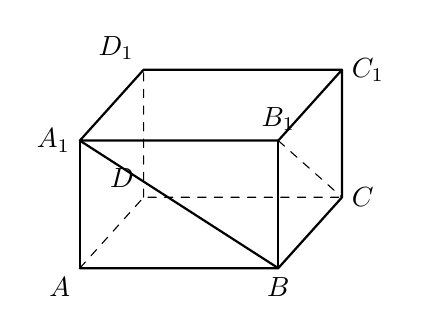
\begin{tikzpicture}[line cap=round,line join=round,scale=0.9]
  \coordinate (A) at (0,0);
  \coordinate (B) at (2.8,0);
  \coordinate (C) at (3.7,1.0);
  \coordinate (D) at (0.9,1.0);
  \coordinate (A1) at (0,1.8);
  \coordinate (B1) at (2.8,1.8);
  \coordinate (C1) at (3.7,2.8);
  \coordinate (D1) at (0.9,2.8);

  % 长方体可见棱与遮挡棱。
  \draw[thick] (A)--(B)--(C)--(C1)--(B1)--(A1)--(D1)--(C1);
  \draw[thick] (A1)--(A) (B1)--(B);
  \draw[dashed] (A)--(D)--(C) (D)--(D1);

  % 题干中的 A_1B 与 B_1C。
  \draw[thick] (A1)--(B);
  \draw[dashed] (B1)--(C);

  \node[below left] at (A) {$A$};
  \node[below] at (B) {$B$};
  \node[right] at (C) {$C$};
  \node[above left] at (D) {$D$};
  \node[left] at (A1) {$A_1$};
  \node[above] at (B1) {$B_1$};
  \node[right] at (C1) {$C_1$};
  \node[above left] at (D1) {$D_1$};
\end{tikzpicture}
\end{center}
\nopagebreak[4]
\Needspace{4\baselineskip}
\textbf{解析}

\Needspace{5\baselineskip}
连接 $A_1D$。因为长方体对面平行，$A_1D\parallel B_1C$，所以异面直线 $A_1B$ 与 $B_1C$ 所成的角等于 $\angle BA_1D$。连接 $BD$，则
\nopagebreak[4]
\[
A_1B=A_1D=\sqrt{4^2+3^2}=5,\qquad BD=\sqrt{4^2+4^2}=4\sqrt2.
\]
\Needspace{5\baselineskip}
由余弦定理，
\nopagebreak[4]
\[
\cos\angle BA_1D=\frac{5^2+5^2-(4\sqrt2)^2}{2\cdot5\cdot5}=\frac9{25}.
\]
因此所求角为 $\arccos\dfrac9{25}$。

\gkanswer{答案：$\arccos\dfrac9{25}$}

\end{answer}
\begin{answer}
\gksolhead{18}{}

\textbf{题目}（本题满分 12 分）：

已知复数 $w$ 满足 $w-4=(3-2w)i$（$i$ 为虚数单位），$z=\dfrac5w+|w-2|$，求一个以 $z$ 为根的实系数一元二次方程。

\Needspace{4\baselineskip}
\textbf{解析}

\Needspace{5\baselineskip}
由 $w-4=(3-2w)i$，得 $w(1+2i)=4+3i$，所以 $w=2-i$。进而
\nopagebreak[4]
\[
z=\frac5{2-i}+|-i|=2+i+1=3+i.
\]
\Needspace{5\baselineskip}
因所求二次方程系数为实数，若一个根为 $3+i$，另一个根必为共轭数 $3-i$。故可取
\nopagebreak[4]
\[
x^2-6x+10=0.
\]

\gkanswer{答案：$x^2-6x+10=0$}

\end{answer}
\begin{answer}
\gksolhead{19}{}

\textbf{题目}（本题满分 14 分）：

本题共有 2 个小题，第 1 小题满分 8 分，第 2 小题满分 6 分。

\Needspace{5\baselineskip}
已知函数
\nopagebreak[4]
\[
f(x)=2\sin\left(x+\frac\pi6\right)-2\cos x,\qquad x\in\left[\frac\pi2,\pi\right].
\]

（1） 若 $\sin x=\dfrac45$，求函数 $f(x)$ 的值；

（2） 求函数 $f(x)$ 的值域。

\Needspace{4\baselineskip}
\textbf{解析}

\Needspace{5\baselineskip}
利用和角公式，
\nopagebreak[4]
\[
f(x)=2\left(\frac{\sqrt3}{2}\sin x+\frac12\cos x\right)-2\cos x
=\sqrt3\sin x-\cos x
=2\sin\left(x-\frac\pi6\right).
\]

\gksubpart{(1)}

\Needspace{5\baselineskip}
$x\in[\frac\pi2,\pi]$ 且 $\sin x=\frac45$，故 $\cos x=-\frac35$，从而
\nopagebreak[4]
\[
f(x)=\frac{4\sqrt3}{5}+\frac35=\frac{4\sqrt3+3}{5}.
\]

\gksubpart{(2)}

$x-\dfrac\pi6\in[\dfrac\pi3,\dfrac{5\pi}6]$，此区间上正弦函数的值域为 $[\dfrac12,1]$，所以 $f(x)$ 的值域为 $[1,2]$。

\gkanswer{答案（1）：$\dfrac{4\sqrt3+3}{5}$}

\gkanswer{答案（2）：$[1,2]$}

\end{answer}
\begin{answer}
\gksolhead{20}{}

\textbf{题目}（本题满分 14 分）：

本题共有 2 个小题，第 1 小题满分 6 分，第 2 小题满分 8 分。

学校科技小组在计算机上模拟航天器变轨返回试验。设计方案如图：航天器运行（按顺时针方向）的轨迹方程为 $\dfrac{x^2}{100}+\dfrac{y^2}{25}=1$，变轨（即航天器运行轨迹由椭圆变为抛物线）后返回的轨迹是以 $y$ 轴为对称轴、$M\left(0,\dfrac{64}{7}\right)$ 为顶点的抛物线的实线部分，降落点为 $D(8,0)$。观测点 $A(4,0)\text{、}B(6,0)$ 同时跟踪航天器。
\nopagebreak[4]
\begin{center}% 2006 年上海春季卷第 20 题：原卷航天器轨迹示意图的矢量重绘。
% 曲线按题设方程绘制；原图为示意图，除题干已给坐标外不引入比例条件。
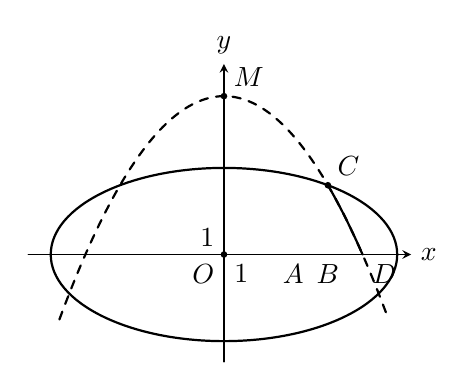
\begin{tikzpicture}[line cap=round,line join=round,x=0.22cm,y=0.22cm,>=stealth]
  % 坐标轴与椭圆运行轨迹 x^2/100+y^2/25=1。
  \draw[->] (-11.3,0)--(10.8,0) node[right] {$x$};
  \draw[->] (0,-6.2)--(0,11.0) node[above] {$y$};
  \draw[thick] (0,0) ellipse (10 and 5);

  % 变轨后的抛物线 y=64/7-x^2/7，原卷以虚线表示。
  \draw[dashed,thick,domain=-9.5:9.5,samples=100,variable=\x]
    plot (\x,{64/7-\x*\x/7});
  % 原卷以实线强调从交点 C 到降落点 D 的运行弧段。
  \draw[thick,domain=6:8,samples=40,variable=\x]
    plot (\x,{64/7-\x*\x/7});

  % 原卷中的基准点与观测点标记。
  \fill (0,0) circle (1.2pt) node[below left] {$O$};
  \fill (0,{64/7}) circle (1.2pt) node[above right] {$M$};
  \fill (6,4) circle (1.2pt) node[above right] {$C$};
  \node[below] at (4,0) {$A$};
  \node[below] at (6,0) {$B$};
  \node[below right] at (8,0) {$D$};
  \node[below] at (1,0) {$1$};
  \node[left] at (0,1) {$1$};
\end{tikzpicture}
\end{center}
\nopagebreak[4]
（1） 求航天器变轨后的运行轨迹所在的曲线方程；

（2） 试问：当航天器在 $x$ 轴上方时，观测点 $A\text{、}B$ 测得离航天器的距离分别为多少时，应向航天器发出变轨指令？

\Needspace{4\baselineskip}
\textbf{解析}

\gksubpart{(1)}

\Needspace{5\baselineskip}
抛物线关于 $y$ 轴对称，顶点为 $M(0,\dfrac{64}{7})$，故可设方程为 $y=ax^2+\dfrac{64}{7}$。又经过降落点 $D(8,0)$，所以
\nopagebreak[4]
\[
0=64a+\frac{64}{7},\qquad a=-\frac17.
\]
变轨后的轨迹方程为 $y=-\dfrac17x^2+\dfrac{64}{7}$。

\gksubpart{(2)}

\Needspace{5\baselineskip}
设变轨点为 $C(x,y)$。它同时在椭圆和返回抛物线上，满足
\nopagebreak[4]
\[
\frac{x^2}{100}+\frac{y^2}{25}=1,\qquad y=-\frac17x^2+\frac{64}{7}.
\]
\Needspace{5\baselineskip}
消去 $x^2$ 得 $4y^2-7y-36=0$，所以 $y=4$ 或 $y=-\dfrac94$。题目要求航天器在 $x$ 轴上方，取 $y=4$；代回椭圆得 $x=\pm6$。返回轨迹为图中的右侧实线部分，降落点为 $D(8,0)$，故取 $C=(6,4)$。因此
\nopagebreak[4]
\[
|AC|=\sqrt{(6-4)^2+4^2}=2\sqrt5,\qquad |BC|=4.
\]
当 $A\text{、}B$ 测得的距离分别为 $2\sqrt5$ 与 $4$ 时，应发出变轨指令。

\gkanswer{答案（1）：$y=-\dfrac17x^2+\dfrac{64}{7}$}

\gkanswer{答案（2）：$|AC|=2\sqrt5$，$|BC|=4$}

\end{answer}
\begin{answer}
\gksolhead{21}{}

\textbf{题目}（本题满分 16 分）：

本题共有 3 个小题，第 1 小题满分 4 分，第 2 小题满分 6 分，第 3 小题满分 6 分。

设函数 $f(x)=|x^2-4x-5|$。

（1） 在区间 $[-2,6]$ 上画出函数 $f(x)$ 的图象；

（2） 设集合 $A=\{x\mid f(x)\geq5\}$，$B=(-\infty,-2]\cup[0,4]\cup[6,+\infty)$。试判断集合 $A$ 和 $B$ 之间的关系，并给出证明；

（3） 当 $k>2$ 时，求证：在区间 $[-1,5]$ 上，$y=k(x+3)$ 的图象位于函数 $f(x)$ 图象的上方。
\nopagebreak[4]
\begin{center}% 2006 年上海春季卷第 21 题：原卷留白坐标网格。
% 单位网格覆盖 [-10,10]×[-10,10]，坐标轴数字按原卷显示到偶数刻度。
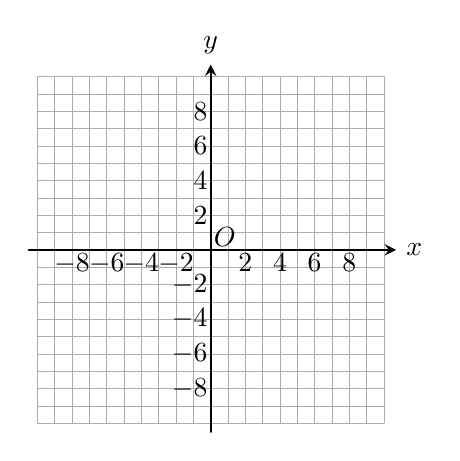
\begin{tikzpicture}[line cap=round,line join=round,x=0.22cm,y=0.22cm,>=stealth]
  \draw[step=1,gray!65,very thin] (-10,-10) grid (10,10);
  \draw[->,thick] (-10.5,0)--(10.7,0) node[right] {$x$};
  \draw[->,thick] (0,-10.5)--(0,10.7) node[above] {$y$};

  \foreach \x in {-8,-6,-4,-2,2,4,6,8}
    \node[below,inner sep=1pt] at (\x,0) {$\x$};
  \foreach \y in {-8,-6,-4,-2,2,4,6,8}
    \node[left,inner sep=1pt] at (0,\y) {$\y$};
  \node[above right,inner sep=1pt] at (0,0) {$O$};
\end{tikzpicture}
\end{center}
\nopagebreak[4]
\Needspace{4\baselineskip}
\textbf{解析}
\nopagebreak[4]
\begin{center}% 2006 年上海春季卷第 21 题（1）：独立解答函数图。
% 与题面空白网格分开；按 f(x)=|x^2-4x-5| 在 [-2,6] 上作图。
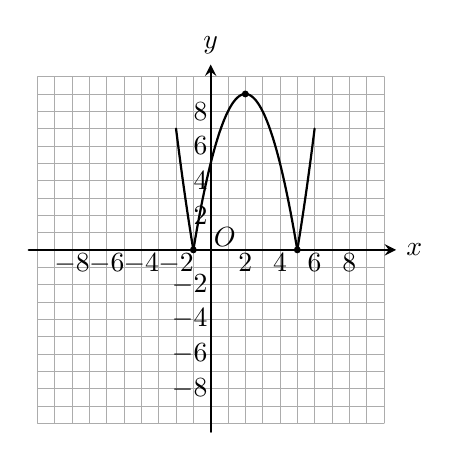
\begin{tikzpicture}[line cap=round,line join=round,x=0.22cm,y=0.22cm,>=stealth]
  \draw[step=1,gray!65,very thin] (-10,-10) grid (10,10);
  \draw[->,thick] (-10.5,0)--(10.7,0) node[right] {$x$};
  \draw[->,thick] (0,-10.5)--(0,10.7) node[above] {$y$};

  \foreach \x in {-8,-6,-4,-2,2,4,6,8}
    \node[below,inner sep=1pt] at (\x,0) {$\x$};
  \foreach \y in {-8,-6,-4,-2,2,4,6,8}
    \node[left,inner sep=1pt] at (0,\y) {$\y$};
  \node[above right,inner sep=1pt] at (0,0) {$O$};

  \draw[thick,domain=-2:-1,samples=40,variable=\x]
    plot (\x,{\x*\x-4*\x-5});
  \draw[thick,domain=-1:5,samples=100,variable=\x]
    plot (\x,{-\x*\x+4*\x+5});
  \draw[thick,domain=5:6,samples=40,variable=\x]
    plot (\x,{\x*\x-4*\x-5});
  \fill (-1,0) circle (1.25pt);
  \fill (2,9) circle (1.25pt);
  \fill (5,0) circle (1.25pt);
\end{tikzpicture}
\end{center}
\nopagebreak[4]
\gksubpart{(1)}

\Needspace{5\baselineskip}
$x^2-4x-5=(x-5)(x+1)$，零点为 $x=-1,5$。因此在 $[-2,-1]\cup[5,6]$ 上原式非负，在 $[-1,5]$ 上原式非正，
\nopagebreak[4]
\[
f(x)=
\begin{cases}
x^2-4x-5,&x\in[-2,-1]\cup[5,6],\\
-x^2+4x+5,&x\in[-1,5].
\end{cases}
\]
两端点 $x=-2,6$ 处 $f(x)=7$；折点为 $(-1,0)$、$(5,0)$；中间抛物线顶点为 $(2,9)$。按这些关键点和区间单调性即可画出图像。

\gksubpart{(2)}

\Needspace{5\baselineskip}
解 $f(x)\geq5$。当 $x^2-4x-5\geq5$ 时，$x^2-4x-10\geq0$，即 $x\leq2-\sqrt{14}$ 或 $x\geq2+\sqrt{14}$；当 $x^2-4x-5\leq-5$ 时，$x(x-4)\leq0$，即 $x\in[0,4]$。故
\nopagebreak[4]
\[
A=(-\infty,2-\sqrt{14}]\cup[0,4]\cup[2+\sqrt{14},+\infty).
\]
因 $2-\sqrt{14}>-2$、$2+\sqrt{14}<6$，所以题设的 $B$ 是 $A$ 的真子集。

\gksubpart{(3)}

\Needspace{5\baselineskip}
当 $x\in[-1,5]$ 时，$x^2-4x-5\leq0$，故 $f(x)=-x^2+4x+5$。令
\nopagebreak[4]
\[
g(x)=k(x+3)-f(x)=x^2+(k-4)x+(3k-5)
=\left(x-\frac{4-k}{2}\right)^2-\frac{k^2-20k+36}{4}.
\]
\Needspace{5\baselineskip}
由于 $k>2$，抛物线顶点横坐标 $\dfrac{4-k}{2}<1$。若 $2<k\leq6$，顶点在 $[-1,5]$ 内，最小值为
\nopagebreak[4]
\[
g_{\min}=-\frac14[(k-10)^2-64]>0,
\]
因为此时 $16\leq(k-10)^2<64$。若 $k>6$，顶点在区间左侧，$g$ 在 $[-1,5]$ 上递增，故最小值在 $x=-1$ 处，$g(-1)=2k>0$。所以全区间内 $k(x+3)-f(x)>0$，直线图像严格位于曲线图像上方。

\gkanswer{答案（1）：按分段表达式绘图}

\gkanswer{答案（2）：$B\subsetneq A=(-\infty,2-\sqrt{14}]\cup[0,4]\cup[2+\sqrt{14},+\infty)$}

\gkanswer{答案（3）：见解析版}

\end{answer}
\begin{answer}
\gksolhead{22}{}

\textbf{题目}（本题满分 18 分）：

本题共有 3 个小题，第 1 小题满分 4 分，第 2 小题满分 8 分，第 3 小题满分 6 分。

已知数列 $a_1,a_2,\cdots,a_{30}$，其中 $a_1,a_2,\cdots,a_{10}$ 是首项为 1，公差为 1 的等差数列；$a_{10},a_{11},\cdots,a_{20}$ 是公差为 $d$ 的等差数列；$a_{20},a_{21},\cdots,a_{30}$ 是公差为 $d^2$ 的等差数列（$d\neq0$）。

（1） 若 $a_{20}=40$，求 $d$；

（2） 试写出 $a_{30}$ 关于 $d$ 的关系式，并求 $a_{30}$ 的取值范围；

（3） 续写已知数列，使得 $a_{30},a_{31},\cdots,a_{40}$ 是公差为 $d^3$ 的等差数列，……，依次类推，把已知数列推广为无穷数列。提出同（2）类似的问题（（2）应当作为特例），并进行研究，你能得到什么样的结论？

\Needspace{4\baselineskip}
\textbf{解析}

\gksubpart{(1)}

首段等差数列首项为 1、公差为 1，故 $a_{10}=10$。第二段有 $a_{20}=a_{10}+10d=10+10d=40$，得 $d=3$。

\gksubpart{(2)}

\Needspace{5\baselineskip}
第三段有 $a_{30}=a_{20}+10d^2=10+10d+10d^2$，所以
\nopagebreak[4]
\[
a_{30}=10(1+d+d^2)=10\left[\left(d+\frac12\right)^2+\frac34\right],\qquad d\neq0.
\]
平方项最小值在 $d=-\dfrac12$ 处取得，符合 $d\neq0$，故值域为 $[\dfrac{15}{2},+\infty)$。

\gksubpart{(3)}

\Needspace{5\baselineskip}
对 $n\geq1$，将每段公差依次取为 $d^n$，可得
\nopagebreak[4]
\[
a_{10(n+1)}=10(1+d+d^2+\cdots+d^n).
\]
\Needspace{5\baselineskip}
先用等比数列公式可写成
\nopagebreak[4]
\[
a_{10(n+1)}=
\begin{cases}
10\dfrac{1-d^{n+1}}{1-d},&d\neq1,\\
10(n+1),&d=1.
\end{cases}
\]
下面讨论固定整数 $n$ 时、参数 $d\in\mathbb R\setminus\{0\}$ 的完整值域。

\Needspace{5\baselineskip}
若 $n$ 为奇数，令 $P_n(d)=1+d+\cdots+d^n$。当 $d\geq0$ 时，$P_n'(d)=1+2d+\cdots+nd^{n-1}>0$。当 $d=-x<0$ 时，利用等比和的导数形式，
\nopagebreak[4]
\[
P_n'(-x)=\frac{1+(n+1)x^n+nx^{n+1}}{(1+x)^2}>0.
\]
故 $P_n$ 在实数上严格递增，且因其为奇数次多项式，值域为 $\mathbb R$；但排除 $d=0$ 后，值 $P_n(0)=1$ 不再取到。因此 $a_{10(n+1)}$ 的值域为 $\mathbb R\setminus\{10\}$。

\Needspace{5\baselineskip}
若 $n$ 为偶数，在 $d>0$ 上 $P_n(d)$ 从 1 严格递增至 $+\infty$。在 $d=-x<0$ 上，
\nopagebreak[4]
\[
P_n(-x)=\frac{1+x^{n+1}}{1+x},\qquad
\frac{d}{dx}P_n(-x)=\frac{(n+1)x^n+nx^{n+1}-1}{(1+x)^2}.
\]
\Needspace{5\baselineskip}
分子随 $x>0$ 严格递增，从 $-1$ 趋于 $+\infty$，且在 $x=1$ 时为 $2n+1>0$，故存在唯一 $x_n\in(0,1)$ 满足 $(n+1)x_n^n+n x_n^{n+1}=1$。此点给出负半轴上的唯一最小值
\nopagebreak[4]
\[
\mu_n=P_n(-x_n)=\frac{1+x_n^{n+1}}{1+x_n}<1,
\]
其中 $x_n<1$ 蕴含 $x_n^{n+1}<x_n$。
并且 $P_n(-x)\to+\infty$ 当 $x\to+\infty$，所以 $P_n$ 在负半轴上的值域为 $[\mu_n,+\infty)$，已包含正半轴分支。于是 $a_{10(n+1)}$ 的值域为 $[10\mu_n,+\infty)$。当 $n=2$ 时，方程 $3x^2+2x^3=1$ 的唯一正根为 $x_2=\dfrac12$，$\mu_2=\dfrac34$，恰得第（2）问的 $[\dfrac{15}{2},+\infty)$。

\gkanswer{答案（1）：$d=3$}

\gkanswer{答案（2）：$a_{30}=10(1+d+d^2)$，值域 $[\dfrac{15}{2},+\infty)$}

\gkanswer{答案（3）：$a_{10(n+1)}=10(1+d+\cdots+d^n)$。固定 $n$ 为奇数时值域 $\mathbb R\setminus\{10\}$；固定 $n$ 为偶数时，令 $x_n>0$ 为 $(n+1)x_n^n+n x_n^{n+1}=1$ 的唯一正根，$\mu_n=\dfrac{1+x_n^{n+1}}{1+x_n}$，值域为 $[10\mu_n,+\infty)$。$n=2$ 时 $x_2=\dfrac12$、$\mu_2=\dfrac34$，与（2）相同}

\end{answer}